% LTeX: language=fr

\chapter{Solutions retenues}










\section{Acquisition forensique}

Il existe deux types de données forensiques: les données volatiles contenues dans la RAM et les données non-volatiles contenues sur le disque, chacune avec ses avantages et ses inconvénients.





\subsection{Données volatiles}

Pour acquérir les données de la RAM, il faut charger un logiciel dans la RAM, ce qui entraîne donc une modification de ces données. De plus, si un rootkit (logiciel malveillant persistant et furtif) est installé sur le système, il peut renvoyer des fausses informations, voir effacer ses traces en supprimant des données à la fois volatiles et non-volatiles comme des fichiers ou des clés de registres. Souvent, on considère que le jeu en vaut la chandelle et on prend ce risque. Cependant, cette décision doit être prise au préalable et pas sur le moment même. \cite{5}

Les outils que j'ai sélectionnés pour la capture de la RAM sont:

\begin{itemize}
    \item \textit{Belkasoft Live RAM Capturer} créé par Belkasoft;
    \item \textit{Magnet RAM Capture} créé par Magnet Forensics;
    \item \textit{FTK Imager} créé par Access Data.
\end{itemize}

\begin{figure}
    \centering
    \makebox[\textwidth]{
        \resizebox{19cm}{!}{
            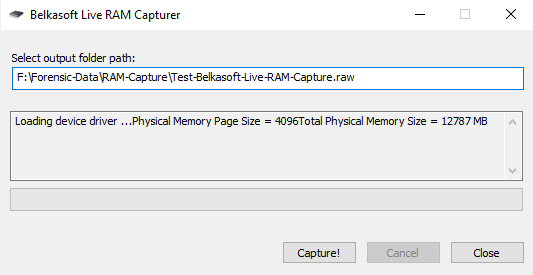
\includegraphics[width=14.45cm]{images/RAM/ram-capture-01.png}
            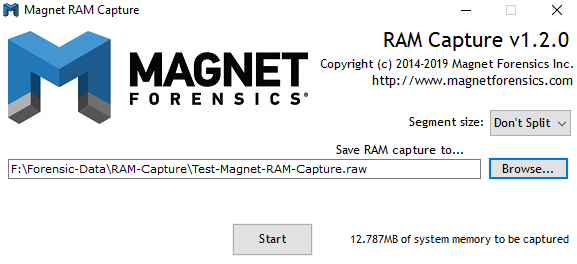
\includegraphics[width=14.45cm]{images/RAM/ram-capture-02.png}
        }
    }
    \caption{Interfaces graphiques des logiciels de capture RAM \textit{Belkasoft Live RAM Capturer} et \textit{Magnet RAM Capturer}.}
    \label{fig:ram-capture-softwares}
\end{figure}

La raison pour laquelle j'ai sélectionné ces trois logiciels est qu'ils ont été créés par des entreprises qui les supportent, mais aussi parce qu'ils sont gratuits. En fait, ces entreprises, fournissent des outils d'analyse forensique payants mais des logiciels d'acquisition de données forensiques gratuits. Ils ont donc tout intérêt à supporter ces logiciels, voir à les améliorer. D'abord, parce que c'est une porte d'entrée pour de nouveaux clients, mais aussi parce qu'en cas de problème, ils risqueraient de perdre des clients déjà acquis.

Parmi ces trois logiciels, Belkasoft Live RAM Capturer et Magnet RAM Capturer sont les plus simples d'utilisation car ils ont une interface extrêmement simple comme vous pouvez le voir sur la figure \ref{fig:ram-capture-softwares}. Mais pour les départager, j'ai aussi effectué des tests: des tests sur un PC de test et des tests sur une machine virtuelle dont j'ai fait une snapshot pour que les conditions soient les plus similaires possibles. Pour cela, j'ai fait la demande pour obtenir un PC de test chez NRB. J'ai ensuite testé l'acquisition de la mémoire vive avec ces logiciels et je les ai analysés avec le module \textit{windows.statistics.Statistics} du logiciel d'analyse \textit{volatility 3}, qui permet de comparer le nombre de pages mémoire invalides.

Le résultat est que \textit{Magnet RAM Capture} avec 141 345 pages invalides est moins bon que de \textit{Belkasoft Live RAM Capturer} avec seulement 46 629 pages invalides. Et ça se remarque d'ailleurs avec l'utilisation du module \textit{windows.pslist.PsList}, lequel montre un processus avec un PID extrêmement haut 104942906544106, et un nom de processus bizarre contenant des caractères unicodes: \texttt{<4{\quem}YJ{\quem\quem}wd{\quem}L!\quem}, ce qui montre une erreur de capture RAM. Ceci montre aussi l'importance d'effectuer une capture RAM avec le moins d'erreurs possible car on en retire de mauvaises informations.

Pour comprendre comment une page peut être est invalide, il faut comprendre le concept de \textit{mémoire virtuelle}. La mémoire virtuelle consiste à diviser la RAM en un certain nombre de pages ayant chacune une adresse. En traduisant les adresses virtuelles et les adresses réelles des pages RAM, le système d'exploitation simplifie l'utilisation de la RAM par les logiciels mais il peut aussi utiliser le mécanisme de swapping, c'est-à-dire utiliser l'espace disque comme extension de la RAM, ceci explique pourquoi la capture RAM est plus grande que la capacité du PC dont on fait l'image. \cite{7} Le module de statistique de Volatility 3 compte une page virtuelle comme invalide lorsque son adresse physique (la traduction de son adresse virtuelle) est invalide. \cite{8} Ça pourrait arriver, par exemple, si le contenu de la RAM change pendant la capture.

% https://thanursan.medium.com/comparison-of-memory-acquisition-software-for-windows-e8c6d981db23
% https://belkasoft.com/ram-capturer

\begin{table}
    \centering
    \begin{tabular}{cccc} \hline
            & \textbf{Belkasoft} & \textbf{Magnet} & \textbf{FTK Imager} \\ \hline
        \textbf{Temps d'acquisition}  & 90 secondes & 180 secondes & 90 secondes \\
        \textbf{VM - Pages invalides} & 60 010 & 2 180 438 & 2 174 110 \\
        \textbf{PC - Pages invalides} & 46 629 & 141 345 & 96 542 \\
        \textbf{RAM utilisée}         & 26.0 KB & 36.9 KB & 57.8 KB \\ \hline
    \end{tabular}
    \caption{Tableau de comparaison des outils de capture de mémoire RAM.}
    \label{tab:ram-capture}
\end{table}

En effectuant des tests et en prenant des mesures précises, j'ai pu arriver au tableau voir figure \ref{tab:ram-capture} qui permet de comparer de manière objective les différents outils et ainsi, de prendre une décision pour sélectionner quel outil devrait être utilisé lors des acquisitions de données volatiles. Mon choix s'est finalement porté sur l'outil de Belkasoft qui a été meilleur que les autres dans presque toutes les catégories. Pour mesurer la RAM utilisée, j'ai lancé les trois logiciels dans une VM dont j'avais pris une snapshot (un instantané) pour que les conditions soient les mêmes et j'ai utilisé Process Explorer pour mesurer la quantité de RAM utilisée comme vous pouvez le voir sur la figure \ref{fig:ram-used-magnet}.

\begin{figure}
    \centering
    \makebox[\textwidth]{
        \resizebox{18cm}{!}{
            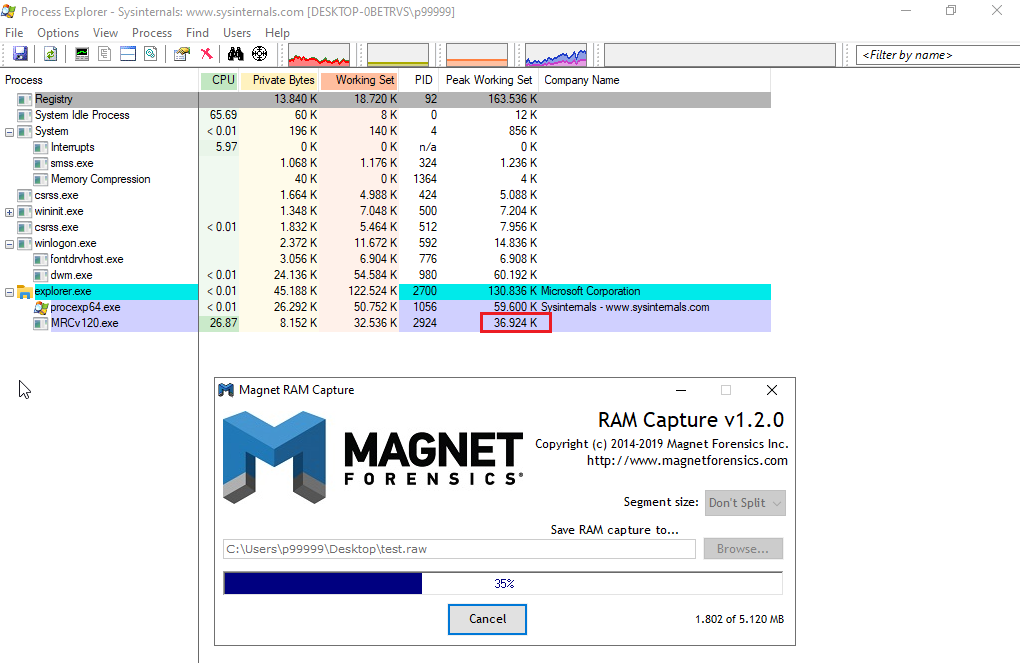
\includegraphics[width=14.45cm]{images/RAM/magnet-test-vm-02.png}
        }
    }
    \caption{Quantité de RAM utilisée par \textit{Magnet RAM Capturer} pendant la capture RAM, mesuré par \textit{Process Explorer} de Sysinternals.}
    \label{fig:ram-used-magnet}
\end{figure}





\subsection{Données non-volatiles}

J'ai sélectionné deux logiciels en utilisant la même réflexion que lors de la sélection de logiciels de capture de la mémoire volatile: que ce soient des logiciels qui sont proposés par des entreprises qui le tiennent à jour, et qu'ils soient gratuits. Les deux logiciels sont les suivants:

\begin{itemize}
    \item \textit{EnCase Forensic Imager} créé par EnCase;
    \item \textit{FTK Imager} créé par Access Data.
\end{itemize}

Malheureusement, je n'ai pas réussi à télécharger Encase Forensic Imager et ils n'ont pas répondu à ma prise de contact. Je n'ai donc pu qu'utiliser FTK Imager pour récupérer une image du disque d'un ordinateur.

\begin{figure}
    \centering
    \makebox[\textwidth]{
        \resizebox{19cm}{!}{
            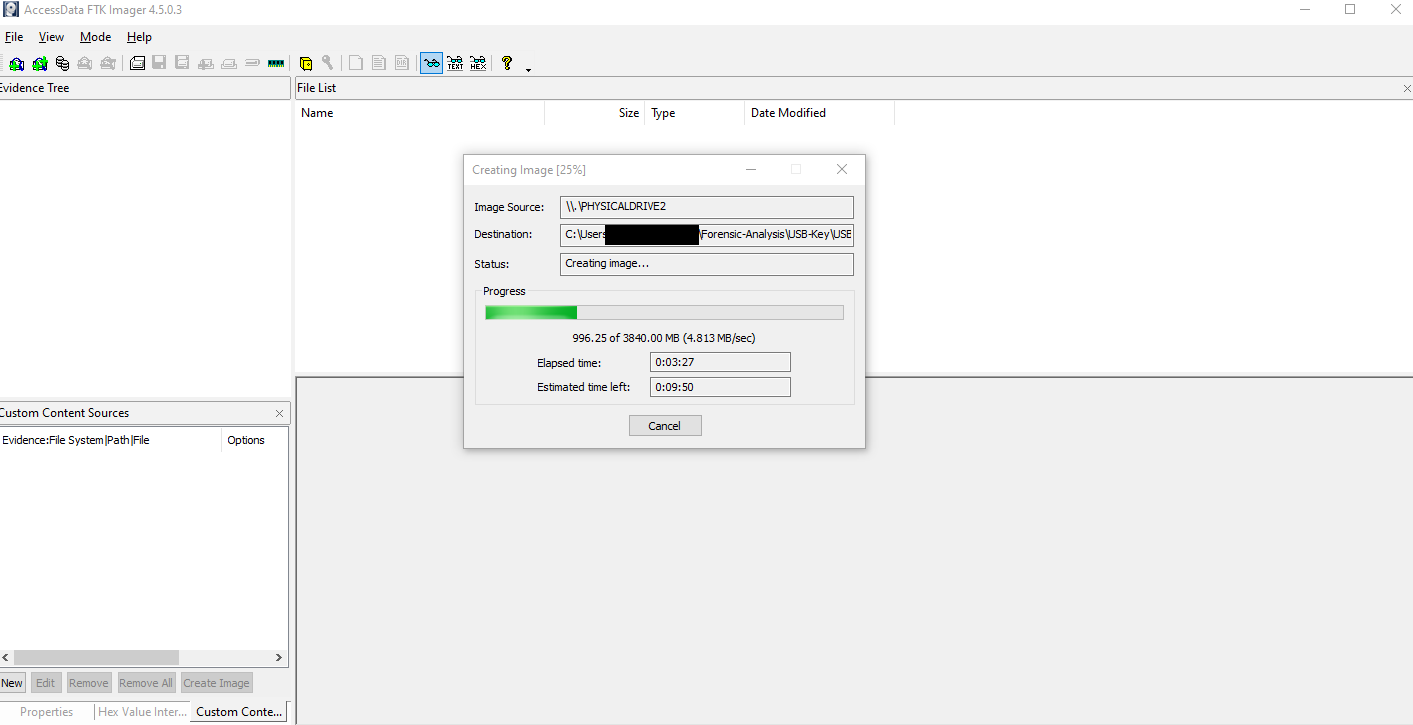
\includegraphics{images/Disque/FTK-Imager.png}
        }
    }
    \caption{Acquisition de la mémoire de masse avec FTK Imager.}
    \label{fig:ftk-imager}
\end{figure}

L'objectif n'est pas de récupérer que les fichiers utilisés par le système d'exploitation mais l'entièreté du disque. Y compris les espaces vides, qui peuvent contenir des données supprimées par un utilisateur ou un logiciel malveillant mais aussi les partitions qui ne sont pas utilisées par le système d'exploitation parce qu'elles pourraient également contenir des informations nécessaires à l'enquête.

Une des difficultés lorsqu'on copie l'entièreté d'un disque, est qu'on peut tomber sur un disque chiffré. Dans ce cas, il faut s'assurer de récupérer la clé de chiffrement. On peut le faire facilement pour les clés BitLocker avec la commande suivante (où il faut remplacer \texttt{<lettre-de-lecteur>} par la lettre représentant le disque dont on veut la clé, par exemple: C, pour le disque principal des PC Windows): \cite{11}

\texttt{manage-bde -protectors <lettre-de-lecteur> -get}










\section{Analyse forensique}





\subsection{Données volatiles}

Pour analyser ces données, il faut bien sûr utiliser des logiciels spécialisés. Il y a peu de logiciels qui permettent de le faire. J'en ai trouvé trois:

\begin{itemize}
    \item Volatility 2 et Volatility 3, un framework ainsi nommé parce qu'il sert à analyser les données volatiles. Volatility 2 est écrit en Python 2 et Volatility 3 en Python 3.
    \item Redline, un outil développé par l'entreprise FireEye.
\end{itemize}

Redline n'a plus été mis à jour depuis avril 2020. Bien qu'il supporte Windows Server 2019 et Windows 10, le logiciel a été incapable d'analyser la dernière version de ce système d'exploitation qui est utilisée dans l'entreprise lors des essais que j'ai réalisés.

Pour ce qui est du framework Volatility, la version 2 n'est plus supportée, tout comme le langage dans lequel elle a été écrite, Python 2. Cependant, Volatility 2 a encore beaucoup de plugins écrits par la communauté qui n'ont pas été réécrits pour fonctionner avec la dernière version. À l'avenir, il faudra bien passer à l'utilisation de Volatility 3, par exemple pour analyser des machines Windows 11 mais en attendant, j'ai décidé de continuer à travailler avec Volatility 2.

\begin{example}
    \hspace{0.45cm} Le \textit{process hollowing} est une sous-technique de l'injection de code malicieux, référencé par l'ID T1055.012 par l'organisation MITRE. Elle est réalisée par des malwares pour éviter d'être détectés par l'anti-virus de la machine. Un processus créé un nouveau processus enfant inoffensif dans un état suspendu, ensuite, il y injecte du code malicieux. \cite{10}

    Le plugin \textit{HollowFind} a été écrit par un chercheur en cybersécurité pour Volatility 2. Il sert à trouver les processus dans lesquels on a injecté du code malicieux avec la méthode de process hollowing. Ce n'est qu'un exemple parmi d'autres de plugins écrits par la communauté qui manquent à la dernière version de Volatility.
\end{example}





\subsection{Données non-volatiles}


\begin{figure}
    \centering
    \makebox[\textwidth]{
        \resizebox{16cm}{!}{
            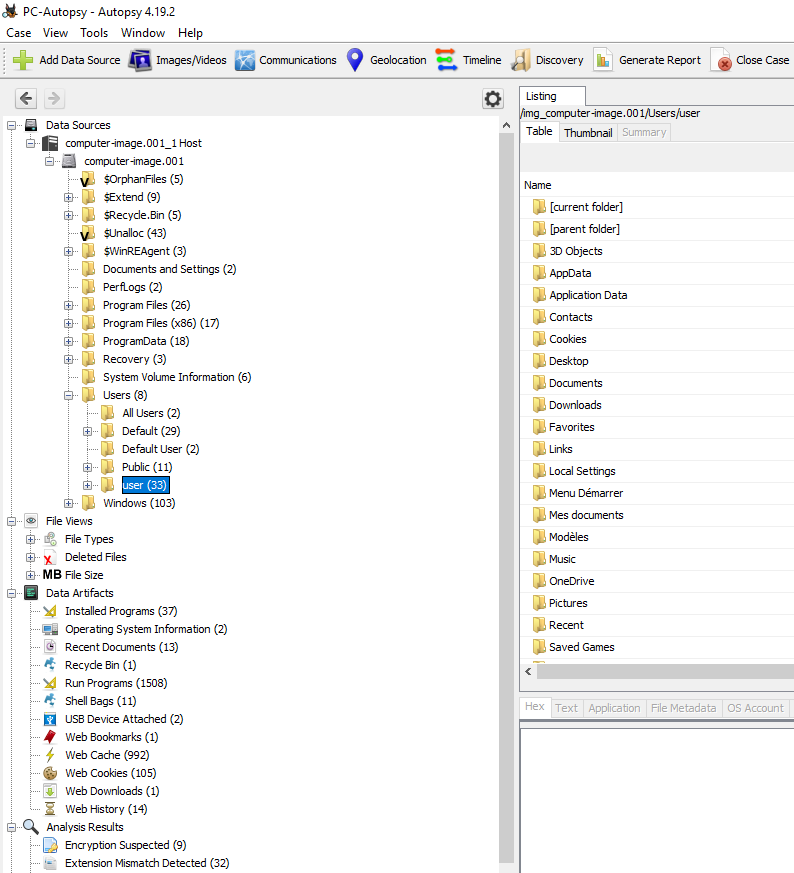
\includegraphics{images/Disque/autopsy-11.png}
        }
    }
    \caption{Autopsy, logiciel d'analyse de mémoire de masse.}
    \label{fig:autopsy-overview}
\end{figure}

Pour analyser les données non-volatiles, il existe plusieurs logiciels gratuits de grande qualité et qui se complètent:

\begin{enumerate}
    \item Autopsy est un logiciel open source qui fonctionne avec une série de modules. Il scanne l'image disque pour lister les volumes et l'arborescence du système de fichier. Il cherche aussi les fichiers supprimés et catégorise les fichiers en fonction de leur taille et de leur extension. Ensuite, on peut choisir de lancer des modules comme l'extracteur d'archives, le détecteur de mauvaise extension, l'analyseur d'emails, etc. Un des plus utiles est le module d'activité récente qui sert à récupérer la liste des documents récents, les données des navigateurs WEB, ainsi que la liste des programmes installés. Autopsy prend beaucoup de temps pour effectuer ces analyses en raison des grandes quantités de données contenues sur un disque. Vous pouvez le voir sur la figure \ref{fig:autopsy-overview}.
    \item Kape et les outils d'Éric Zimmerman fonctionnent de concert pour récupérer des artefacts forensiques de grande importance d'une machine et les analyser. Par exemple, on peut utiliser Kape pour récupérer la MFT (la \textit{master file table}, index principal du système de fichier NTFS) et en normaliser les données pour ensuite les analyser avec l'outil \textit{Timeline Explorer} d'Éric Zimmerman. On peut aussi utiliser Kape pour récupérer les registres et les logs de registres afin de les nettoyer puis les analyser avec l'outil \textit{Registry Explorer} de Zimmerman.
    \item Splunk est un outil SIEM (\textit{Security Information and Event Management}) qui sert à analyser les logs. Un log est l'enregistrement d'un évènement qui s'est produit sur un système informatique, par exemple: lorsqu'une clé USB a été branchée ou débranchée. Cet outil est déjà en place dans l'entreprise.
    \item Chainsaw est un outil d'analyse de logs Windows open source créé par l'entreprise F-Secure (figure \ref{fig:chainsaw}). Il utilise un ensemble de règles pour déterminer si des événements pertinents du point de vue de la cybersécurité se sont produits comme du mouvement latéral, c'est-à-dire le déplacement d'un attaquant au sein du réseau de l'entreprise.
    \item Thor Lite est un scanner anti-virus gratuit qui a bien sûr des limitations par rapport à la version payante parce qu'avec la version Lite, on peut scanner les exécutables mais pas certains types de fichiers comme les raccourcis Windows (d'extension \textit{.lnk}). Dans sa version payante, il va également aller scanner les clés de registres et autres endroits où les malwares peuvent aller se cacher. C'est cependant un outil déjà très utile dans sa version Lite puisqu'il nous sert à repasser là où d'autres anti-virus, comme Windows Defender, ont échoué.
\end{enumerate}

\begin{figure}
    \centering
    \makebox[\textwidth]{
        \resizebox{19cm}{!}{
            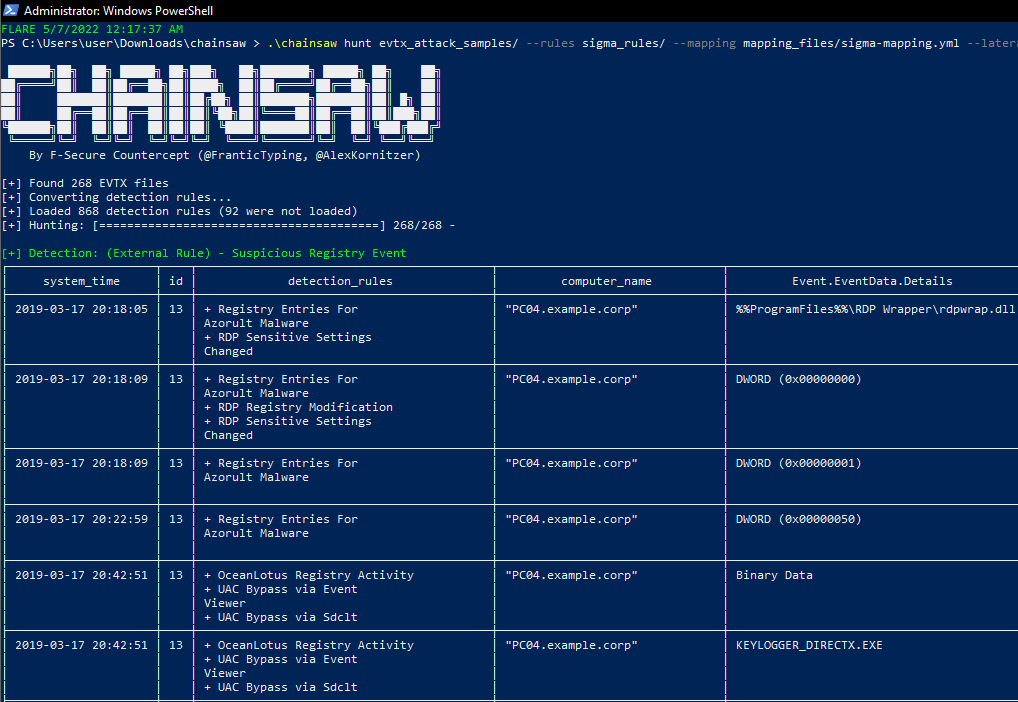
\includegraphics{images/Disque/chainsaw-03.png}
        }
    }
    \caption{Utilisation de chainsaw sur des logs Windows de test.}
    \label{fig:chainsaw}
\end{figure}

Les logiciels se complètent parce qu'on peut les utiliser pour naviguer dans le système de fichiers, analyser les fichiers supprimés, les dossiers consultés, mais aussi trouver les logiciels malveillants dans le système de fichiers, essayer de comprendre ce que l'acteur malveillant a fait sur le système, etc. Aucun d'entre eux ne peut tout faire seul mais en les combinant, on arrive à récupérer un maximum d'informations pour nous aider à comprendre et résoudre l'incident.

Malheureusement, ces outils ne peuvent pas tous analyser l'image disque directement. Certains le peuvent, comme Autopsy, mais dans le cas où le disque de la machine à analyser a été chiffré, les informations récupérées seront très pauvres. On pourrait récupérer la liste des partitions mais aucune information venant du système de fichiers parce que ces informations sont illisibles. Dans ce cas, il faut utiliser l'outil \textit{Arsenal Image Mounter} qui est un logiciel gratuit (avec une version payante) permettant de monter l'image disque comme si on venait de brancher une clé USB. Le logiciel permet de monter l'image en read-only (figure \ref{fig:arsenal-image-mounter}). Une fois montée, on peut facilement sélectionner le disque dans l'explorateur de fichiers pour le déchiffrer avec la clé BitLocker (figure \ref{fig:bitlocker}).

\begin{figure}
    \centering
    \makebox[\textwidth]{
        \resizebox{18cm}{!}{
            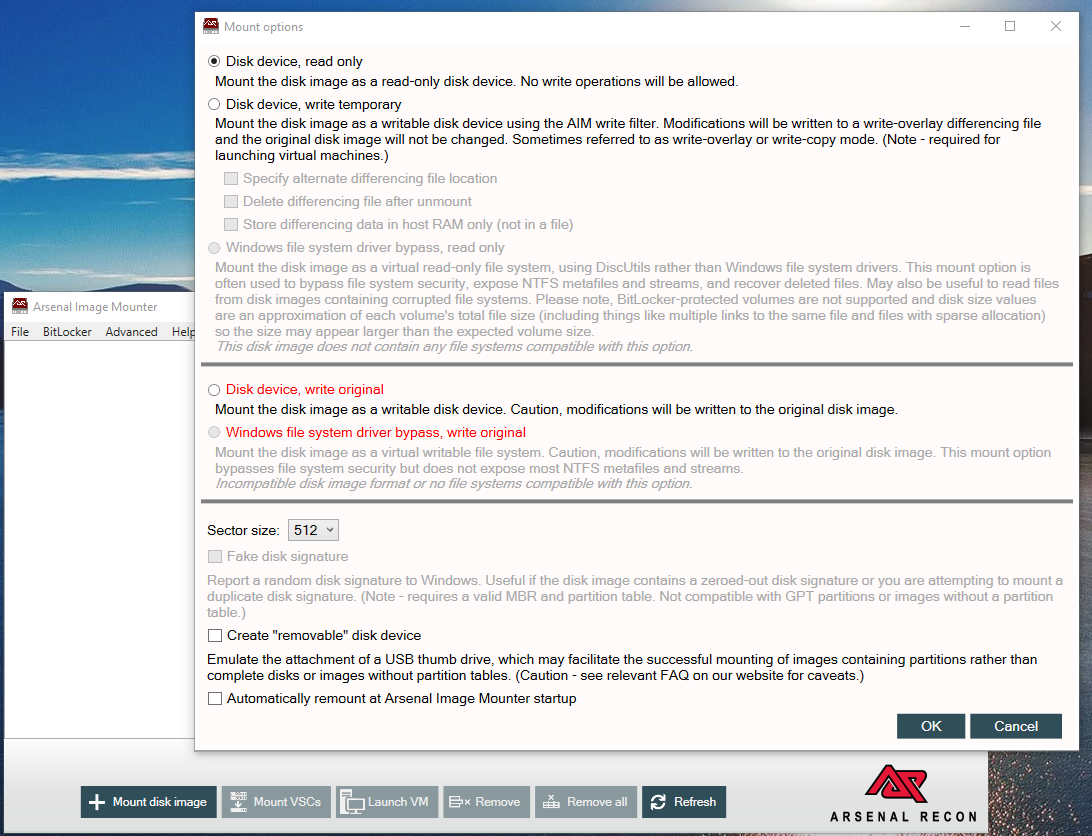
\includegraphics{images/Disque/arsenal-image-mounter-01.png}
        }
    }
    \caption{Montage d'une image disque en lecture seule avec Arsenal Image Mounter.}
    \label{fig:arsenal-image-mounter}
\end{figure}

\begin{figure}
    \centering
    \makebox[\textwidth]{
        \resizebox{10cm}{!}{
            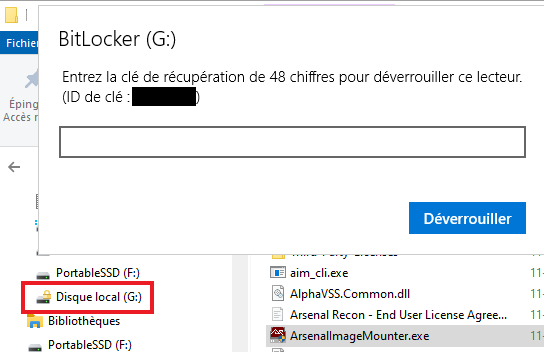
\includegraphics{images/Disque/arsenal-image-mounter-04.png}
        }
    }
    \caption{Déchiffrement d'une image disque montée chiffrée avec BitLocker.}
    \label{fig:bitlocker}
\end{figure}





\subsection{Données externes}

L'analyse forensique ne se contente généralement pas à une seule machine mais elle s'étend également à un ensemble d'appareils qui font partie du système informatique. Par exemple, c'est aussi très important d'exporter les données provenant des pare-feux, des proxys, des solutions de monitoring ou de management d'endpoints comme Microsoft EDR. En particulier si les informations provenant de ces appareils ne sont conservés que sur de courtes périodes. Leur analyse, généralement à l'aide d'un outil de SIEM comme Splunk peut changer le cours d'une enquête forensique ou tout du moins apporter beaucoup d'informations.

\begin{example}
    \hspace{0.45cm} Dans le cas où la machine d'un développeur a été compromise, il est naturel de suspecter qu'il y a pu y avoir du mouvement latéral, c'est-à-dire, que l'attaquant s'est déplacé dans le réseau en compromettant d'autres postes de travail ou des serveurs auxquels la victime a accès. En analysant les logs du pare-feu et des serveurs, si on ne trouve aucune connexion pendant la période d'infection, ça peut indiquer que la contamination est restée localisée.

    De plus, si l'attaquant a été furtif, il a potentiellement effacé les traces de son passage sur le système au fur et à mesure qu'il effectuait des actions. Dans ce cas, c'est particulièrement important de récupérer les logs des autres appareils ou d'aller les recherches dans l'outil de monitoring comme Microsoft EDR ou Splunk.
\end{example}










\section{Solution de sandbox}

Sandbox veut dire \textit{bac à sable} en anglais. Ce terme est utilisé en informatique pour désigner un environnement isolé dans lequel on peut faire tourner un logiciel sans qu'il y ait de conséquences négatives sur le reste de l'ordinateur. Grâce à ces sandboxes, un utilisateur peut exécuter un programme potentiellement dangereux sans mettre en danger ses données, ni endommager son système. Par abus de langage, on appelle aussi \textit{sandbox}, un logiciel qui analyse automatiquement le comportement des logiciels et documents malveillants dans un environnement isolé. Ce logiciel reçoit en entrée un fichier et le place dans une sandbox pour le \textit{détonner}. En sortie, ce logiciel donnera un rapport dans lequel le comportement du fichier est analysé. Ces sandboxes contiennent un système d'exploitation, souvent \textit{Windows}, et des logiciels régulièrement exploités par des acteurs malveillants comme Adobe Acrobat, Microsoft Excel ou Microsoft Word. Les logiciels malveillants que nous cherchons à analyser sont appelés \textit{malwares} pour \textit{malicious software} et \textit{maldoc}, abréviation de \textit{malicious document}, lorsqu'ils sont inclus dans un document PDF, Word ou autre.

Comme expliqué, certains produits appelés sandbox ne correspondent pas à ce que nous cherchons, parmi ceux-ci, il y a: Microsoft Sandbox, Sandboxie, Shade Sandbox, etc. Parmi les autres critères de comparaison que nous allons utiliser, il y a:
\begin{itemize}
    \item Le \textit{prix}, si certaines sandboxes sont gratuites et open source, les solutions commerciales peuvent coûter de quelques centaines d'euros à plusieurs dizaines de milliers d'euros par an.
    \item S'il existe une \textit{version communauté gratuite}, en général, c'est une version restreinte et pour obtenir toutes les fonctionnalités, il faut passer à la version payante.
    \item Si c'est une \textit{solution indépendante} ou si elle fait partie d'une solution d'EDR (Endpoint Detection and Response) ou d'une suite antivirus.
    \item Les \textit{plateformes supportées}, c'est-à-dire si on peut analyser des malwares qui ne tournent que sur Windows, ou si on peut également analyser des malwares qui tournent sur Linux, macOS ou Android.
    \item Le \textit{service proposé}, est-ce qu'on y a accès uniquement via un SaaS (Software as a Service) ? Est-ce une solution hardware ou une VM qu'on peut installer sur un hyperviseur ou dans le cloud ?
    \item Peut-on \textit{interagir manuellement} avec l'analyse ? Certains malwares requièrent une interaction humaine pour s'activer.
    \item Est-ce possible d'exporter les données forensiques de la sandbox, comme une capture de la RAM ou un enregistrement des paquets échangés sur le réseau pour une analyse forensique manuelle plus poussée ?
\end{itemize}

En fin de compte, j'ai décidé de diviser les solutions en trois catégories en fonction du prix:
\begin{enumerate}
    \item Les sandboxes gratuites (table \ref{tab:sandbox-gratuites}).
    \item Les sandboxes qui ont une version communauté gratuite (table \ref{tab:sandbox-community}).
    \item Les sandboxes qui ne possèdent qu'une version payante (table \ref{tab:sandbox-payantes}).
\end{enumerate}

Finalement, nous avons choisi de garder la sandbox \textit{CAPEv2} pour plusieurs raisons:
\begin{enumerate}
    \item Parce que c'est une solution open source gratuite.
    \item Parce qu'on peut la faire tourner \textit{on premise}, c'est-à-dire sur l'infrastructure NRB pour éviter que des informations sensibles ne puissent fuiter.
    \item Parce qu'elle supporte à la fois Windows et Linux qui sont les deux systèmes utilisés dans l'entreprise.
    \item Parce qu'elle contient beaucoup de fonctionnalités avancées comme un débogueur intégré, ce qui permet de contrôler le flux d'exécution d'un malware qui tenterait d'échapper à l'analyse automatique.
    \item Parce que c'est un projet qui est maintenu par une communauté de développeurs active.
\end{enumerate}

Sur le tableau de comparaison \ref{tab:sandbox-gratuites}, la sandbox \textit{Cuckoo} semble posséder plus de caractéristiques positives que \textit{CAPEv2}, alors pourquoi ne pas la prendre ? Le problème des solutions open source est qu'il faut qu'elles trouvent des développeurs motivés pour rester à jour, ce qui ne semble pas être le cas de Cuckoo. Par exemple, cette sandbox est toujours codée dans le langage de programmation python 2 qui n'est lui-même plus supporté par des développeurs. Ce manque de soutien de la part de la communauté peut entraîner des risques de sécurité si on trouve des vulnérabilités dans la sandbox, ils risquent de ne pas être corrigés.

En choisissant CAPEv2, qui est un \textit{fork} (une copie du code en quelque sorte) de Cuckoo et donc possède la même architecture logicielle et la même API (\textit{application programming interface} en anglais), j'ai choisi une sorte de "Cuckoo amélioré" parce que les développeurs en ont modifié le code pour le passer sous python 3 (la version actuelle de python) et y ont ajouté des fonctionnalités. Cependant, ils ont arrêté de faire des tests pour supporter des sandboxes Android.

La sandbox Cuckoo3 est également un fork de Cuckoo qui a simplement fait passer le logiciel sous python 3 mais sans ajouter de nouvelles fonctionnalités, il en a même perdu comme le support du système d'exploitation Android. Il a malgré cela l'avantage d'être soutenu par le CERT de l'Estonie (CERT est l'acronyme de Computer Emergency Response Team). DRAKVUF Sandbox est une sandbox créée par un autre CERT, celui de la Pologne. Son grand avantage est qu'il ne fait pas tourner d'agent sur la machine virtuelle imbriquée mais qu'il va monitorer le comportement du malware depuis l'extérieur via l'hyperviseur, ce qui le rend beaucoup plus difficile à détecter par le malware. En revanche, ses fonctionnalités sont moins complètes que d'autres Sandbox comme CAPE.

\newpage

\begin{tikzpicture}[remember picture, overlay]
    \node () [text width=20cm] at ($(current page.center)+(0,8.5)$) {
        \begin{table}[H]
            \centering
            \begin{tabular}{cccccc} \hline
                    & \textbf{Cuckoo} & \textbf{CAPEv2} & \textbf{Limon} & \textbf{Cuckoo3} & \textbf{Drackvuf} \\ \hline
                \textbf{Solution indépendante} & \oui & \oui & \oui & \oui & \oui \\ \hline
                \textbf{SaaS}       & \oui & \oui & \non & \non & \non \\
                \textbf{Cloud}      & \oui & \oui & \oui & \oui & \oui \\
                \textbf{Hardware}   & \non & \non & \non & \non & \non \\ \hline
                \textbf{Windows}    & \oui & \oui & \non & \oui & \oui \\
                \textbf{Linux}      & \oui & \oui & \oui & \oui & \non \\
                \textbf{Android}    & \oui & \non & \non & \non & \non \\
                \textbf{macOS}      & \oui & \oui & \non & \non & \non \\ \hline
                \textbf{Interaction manuelle} & \oui & \oui & \non & \oui & \oui \\
                \textbf{Export de données forensiques} & \oui & \oui & \oui & \oui & \oui \\ \hline
            \end{tabular}
            \caption{Tableau de comparaison des sandboxes gratuites.}
            \label{tab:sandbox-gratuites}
        \end{table}
    };
    \node () [text width=20cm] at ($(current page.center)+(0,1.5)$) {
        \begin{table}[H]
            \centering
            \begin{tabular}{ccccc} \hline
                    & \textbf{Joe Sandbox} & \textbf{Falcon} & \textbf{any.run} & \textbf{Metadefender} \\ \hline
                \textbf{Solution indépendante} & \oui & \oui & \oui & \oui \\ \hline
                \textbf{SaaS}       & \oui & \oui & \oui & \oui \\
                \textbf{Cloud}      & \oui & \non & \non & \non \\
                \textbf{Hardware}   & \non & \non & \non & \non \\ \hline
                \textbf{Windows}    & \oui & \oui & \oui & \oui \\
                \textbf{Linux}      & \oui & \oui & \non & \non \\
                \textbf{Android}    & \oui & \oui & \non & \non \\
                \textbf{macOS}      & \oui & \oui & \non & \non \\ \hline
                \textbf{Interaction manuelle} & \non & \non & \oui & \non \\
                \textbf{Export de données forensiques} & \oui & \oui & \oui & \non \\ \hline
            \end{tabular}
            \caption{Tableau de comparaison des sandboxes avec une version communauté gratuite.}
            \label{tab:sandbox-community}
        \end{table}
    };
    \node () [text width=20cm] at ($(current page.center)+(0,-6.50)$) {
        \begin{table}[H]
            \centering
            \begin{tabular}{ccccccc} \hline
                    & \rothead{\textbf{Symantec}} & \rothead{\textbf{Kaspersky}} & \rothead{\textbf{McAfee}} & \rothead{\textbf{Fireye}} & \rothead{\textbf{Trend Micro}} & \rothead{\textbf{Cisco TG}} \\ \hline
                \textbf{Solution indépendante} & \non & \non & \non & \non & \oui & \oui \\ \hline
                \textbf{SaaS}       & \oui & \non & \non & \non & \non & \non \\
                \textbf{Cloud}      & \oui & \non & \oui & \non & \oui & \oui \\
                \textbf{Hardware}   & \oui & \oui & \oui & \oui & \oui & \oui \\ \hline
                \textbf{Windows}    & \oui & \oui & \oui & \oui & \oui & \oui \\
                \textbf{Linux}      & \non & \non & \non & \non & \non & \non \\
                \textbf{Android}    & \oui & \oui & \oui & \non & \oui & \non \\
                \textbf{macOS}      & \non & \non & \non & \oui & \oui & \non \\ \hline
                \textbf{Interaction manuelle} & \non & \non & \oui & \oui & \non & \oui \\
                \textbf{Export de données forensiques} & \non & \oui & \oui & \non & \non & \oui \\ \hline
            \end{tabular}
            \caption{Tableau de comparaison des sandboxes payantes.}
            \label{tab:sandbox-payantes}
        \end{table}
    };
\end{tikzpicture}

\newpage

L'installation de CAPE est une tâche ardue mais son utilisation est plus aisée. Elle se fait via une interface web (figure \ref{fig:cape-01}) sur laquelle il suffit de cliquer sur le bouton \textit{Submit} puis de choisir le fichier qui sera ensuite testé automatiquement dans la machine virtuelle Windows qui sera recréée pour chaque échantillon soumis à partir d'une snapshot. Une snapshot étant un instantané de la machine à un moment T pour éviter que les conditions soient toujours les mêmes peu importe l'ordre de soumissions. En effet, si on soumet un rootkit deux fois dans une machine qui n'a pas été restaurée, la première fois, il sera détecté comme malicieux mais la seconde, il restera indétecté parce que la première installation cachera le comportement malicieux du second.

Une fois l'analyse effectuée, on peut en voir les résultats avec un résumé coloré comme sur la figure \ref{fig:cape-01} où les trouvailles les plus importantes sont exposées avec des couleurs indiquant leur dangerosité potentielle. On peut aussi voir le détail des fichiers ou des clés de registres ouverts et modifiés. Ou encore récupérer le dump des processus malicieux ou le dump réseau (fichier pcap contenant tous les paquets réseau) pour analyse avec wireshark par exemple.

\begin{figure}
    \centering
    \makebox[\textwidth]{
        \resizebox{18cm}{!}{
            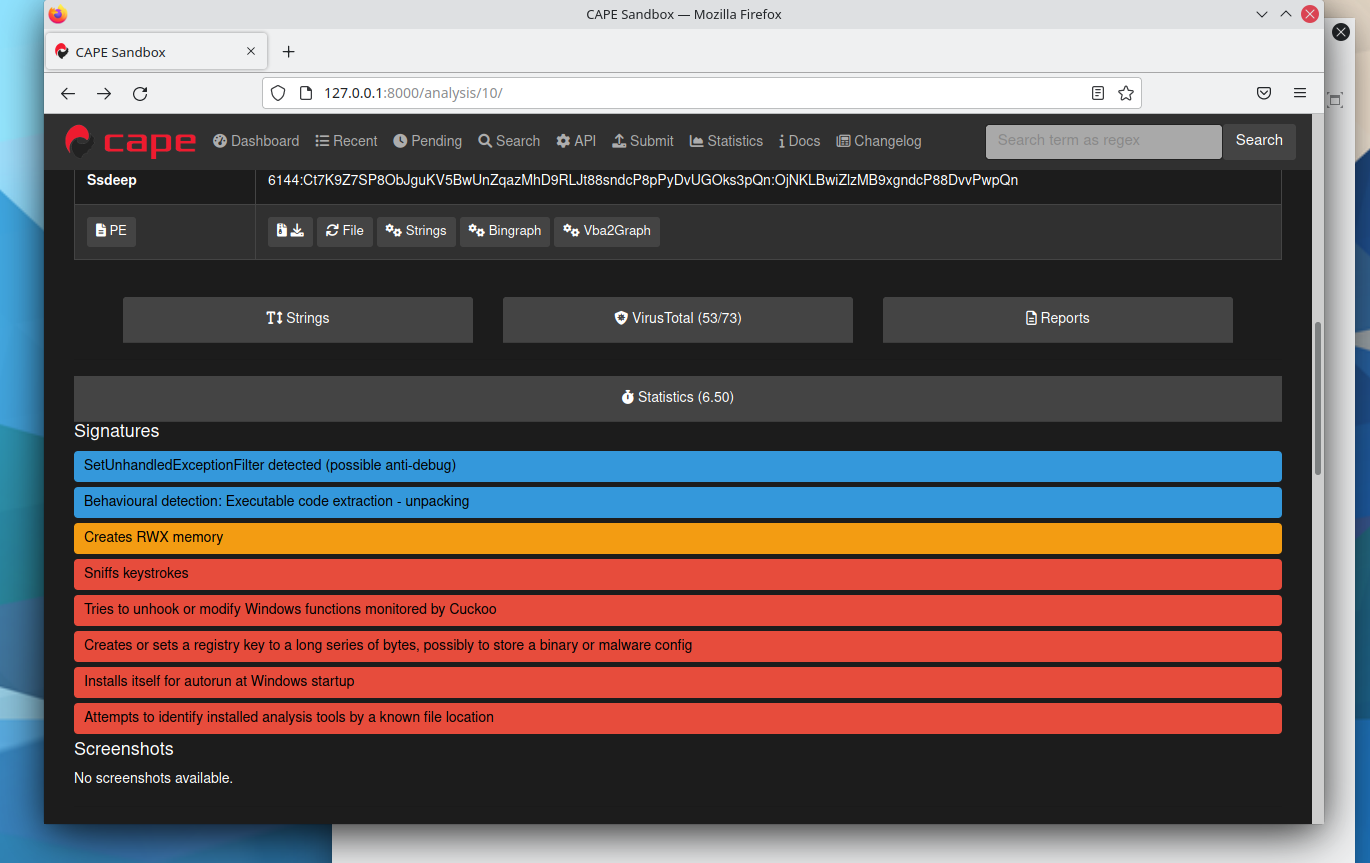
\includegraphics{images/malware/cape-sandbox-exemple.png}
        }
    }
    \caption{Résultats de l'analyse dynamique automatique d'un exécutable avec CAPE Sandbox.}
    \label{fig:cape-01}
\end{figure}

Malheureusement, la machine virtuelle imbriquée lancée par CAPE Sandbox plante complètement (voir figure \ref{fig:sandbox-fail}) lorsqu'on essaie d'analyser un document Office, ce qui n'est pas le cas lorsqu'on essaie d'analyser d'autres types de documents comme des exécutables ou des fichiers PDF. Après plusieurs jours de travail pour essayer de corriger le problème avec Excel, j'ai essayé de passer sur Libre Office. Bien que ça évite le fait que la sandbox affiche un écran bleu, l'analyse ne s'effectuait pas correctement. À nouveau, après plusieurs jours, j'ai dû mettre de côté ce problème pour continuer sur le reste du travail.

\begin{figure}
    \centering
    \makebox[\textwidth]{
        \resizebox{15cm}{!}{
            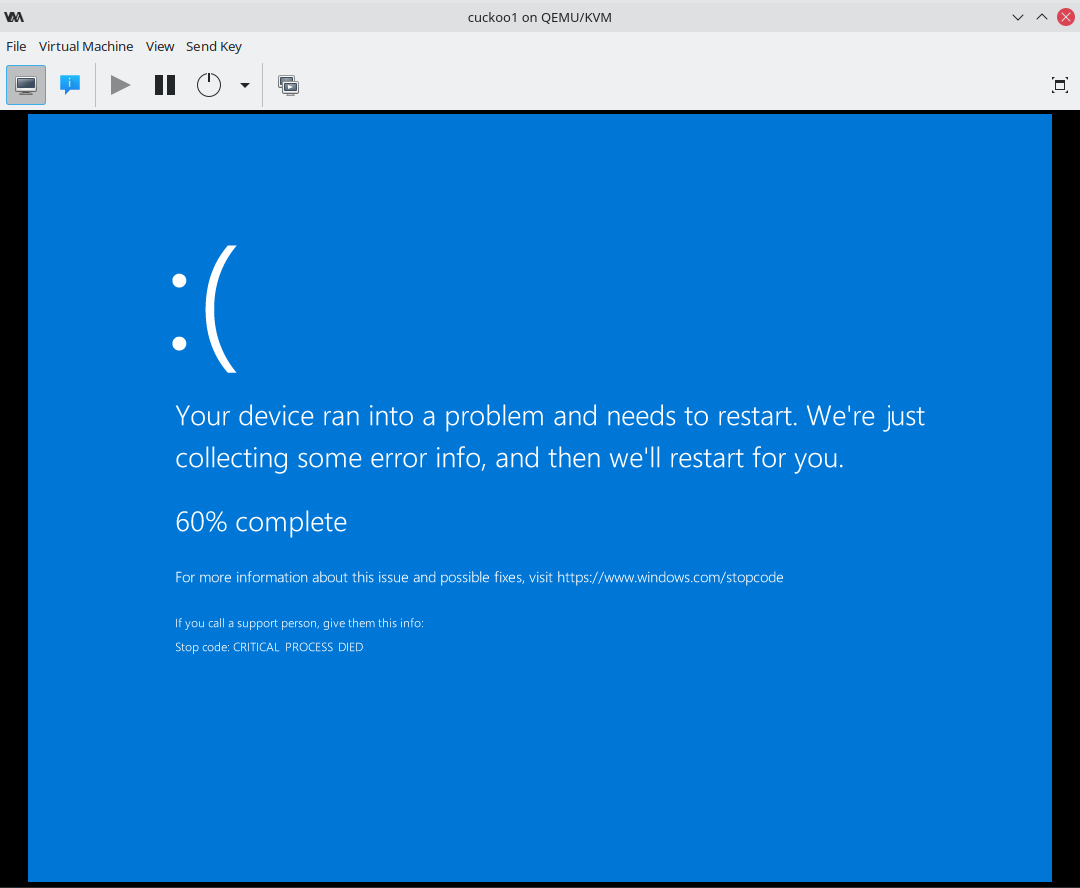
\includegraphics{images/malware/excel-blue-screen-of-death.png}
        }
    }
    \caption{La VM imbriquée plante lorsqu'on essaie d'analyser un document Office.}
    \label{fig:sandbox-fail}
\end{figure}










\section{Analyse de malwares}

Pour analyser les logiciels et documents malveillants, plus communément appelés malwares, j'ai commencé en listant une série d'outils. J'y ai mis des outils d'analyse de documents PDF, d'autres pour analyser les documents Office XML (ceux qui ont une extension terminant par x comme .docx ou .xlsx), les documents Office binaire (les anciens formats avec les extensions .doc, .xls, etc.), les exécutables PE, et encore d'autres. Mais ça rend l'analyse un malware complexe parce qu'il faut maîtriser un grand nombre d'outils pour réussir à analyser tous les types possibles. La solution est d'utiliser la plateforme automatisée \textit{FAME} dévelopée par le CERT (Computer Emergency Response Team) de la Société Générale. C'est l'acronyme de \textit{FAME Automates Malware Evaluation}.

\begin{figure}
    \centering
    \makebox[\textwidth]{
        \resizebox{18cm}{!}{
            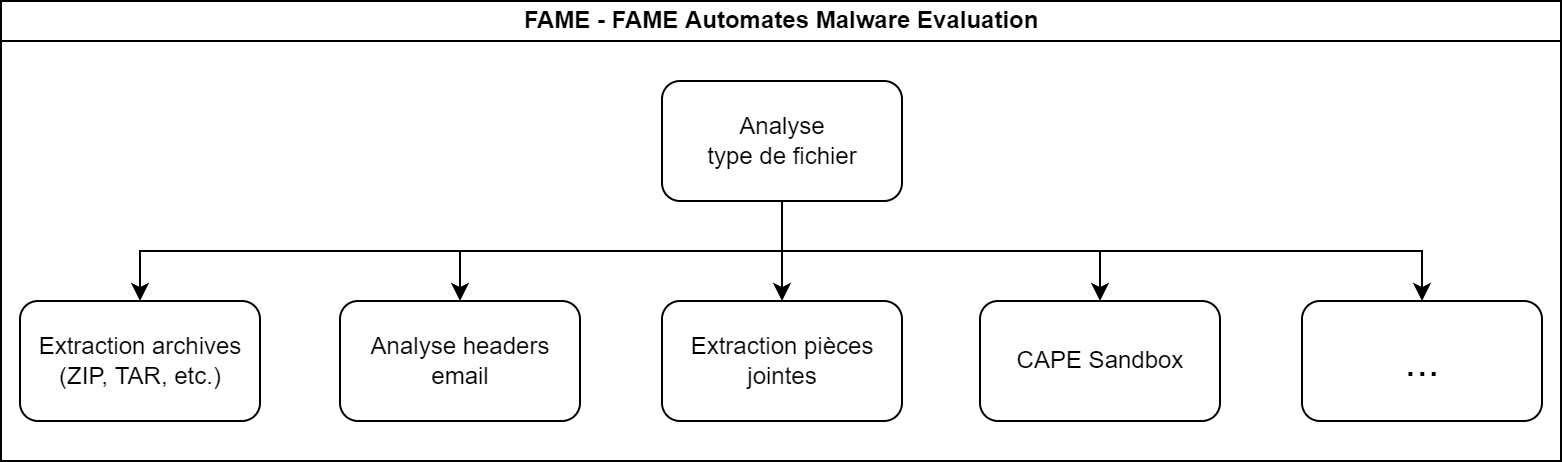
\includegraphics{images/fame-malware-analysis/fame.png}
        }
    }
    \caption{Schéma montrant le fonctionnement de FAME.}
    \label{fig:fame-explanation}
\end{figure}

Comme le montre le schéma sur la figure \ref{fig:fame-explanation}, quand on soumet un fichier à la plateforme, elle commence par déterminer son type afin de décider quels modules vont être lancés. Par exemple, dans le cas d'un document Excel, FAME va lancer à la fois un module d'analyse des métadonnées, un module d'analyse des macros Office, un module d'aperçu qui va générer des images montrant le contenu du document, ainsi que la sandbox pour effectuer une analyse dynamique en simulant l'ouverture du document Excel comme un utilisateur réel le ferait pour voir les actions que les macros vont effectuer sur le système.

Comme vous l'aurez compris, FAME fonctionne avec une série de modules dont un module qui interagit avec la sandbox pour soumettre le fichier malicieux et récupérer les résultats. Il n'y a pas de module fonctionnant avec CAPE, la sandbox choisie et installée dans l'infrastructure d'analyse. Cependant, il y a des modules adaptés à la sandbox Cuckoo dont CAPE est un fork. Ça veut dire qu'on peut facilement adapter le code d'un de ces modules pour le faire fonctionner avec la sandbox déjà installée.

L'utilisation de cette plateforme apporte deux grands avantages:
\begin{itemize}
    \item Elle permet de gagner du temps lorsqu'il y a beaucoup de petites analyses à effectuer. Par exemple, s'il y a une dizaine de cas de phishing à analyser avec parfois plusieurs pièces jointes par email, l'utilisation de FAME permet de gagner du temps en automatisant l'analyse. En fait, en temps normal, un analyste n'aurait peut-être pas le temps d'effectuer toutes les analyses et les domaines malveillants utilisés par les adversaires ne seraient probablement pas bloqués. En libérant du temps, l'analyse peut-être plus poussée et ça renforce la sécurité de l'entreprise.
    \item Cette plateforme peut aussi servir dans les investigations forensiques plus poussées où on a réussi à identifier le malware. Grâce à cette plateforme, on peut ainsi obtenir une première analyse ou effectuer un premier tri s'il y a beaucoup de fichiers à analyser. Il faudra malgré tout effectuer une analyse manuelle si c'est nécessaire pour le bon avancement de l'enquête.
\end{itemize}

\begin{figure}
    \centering
    \makebox[\textwidth]{
        \resizebox{16cm}{!}{
            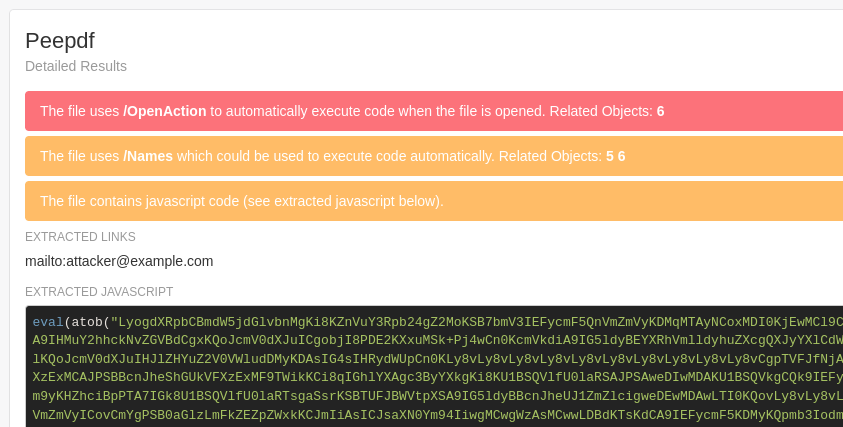
\includegraphics{images/malware/fame-pdf.png}
        }
    }
    \caption{Analyse d'un fichier PDF par FAME qui en extrait les liens, le javascript et émet des alertes.}
    \label{fig:fame-pdf-analysis}
\end{figure}

\begin{example}
    \hspace{0.45cm} Par exemple, si un employé du département des ressources humaines reçoit un PDF vérolé par email, il se peut qu'il remarque une activité suspecte et le signale, ou bien que l'outil de monitoring de sa machine (comme \textit{Microsoft Endpoint Detection and Response}) le détecte. À partir de là, un analyste peut demander à récupérer le PDF ou l'email. En le soumettant dans FAME, on va avoir un résultat comme sur la figure \ref{fig:fame-pdf-analysis} qui montre bien que le document est malicieux. En analysant le code manuellement, on pourrait retrouver des indicateurs de compromissions comme des adresses IP ou des noms de domaines qu'on pourrait ensuite ajouter sur une blacklist pour éviter d'être compromis à l'avenir. Ces indicateurs servent aussi à chercher si d'autres machines n'ont pas déjà été compromises en regardant dans l'outil de SIEM (comme \textit{Splunk}) pour vérifier si d'autres machines les ont déjà contactés.
\end{example}










\section{Distributions de forensique}

Une distribution est un ensemble de logiciels groupés ensemble, ça vient de l'anglais \textit{software distribution}. Et donc une distribution orientée forensique est une collection de logiciels utilisés dans le processus forensique. Ce terme s'applique plus généralement au système d'exploitation Linux mais dans notre cas, il y a aussi des distributions Windows qui sont donc des ensembles d'outils regroupés ensemble qui ne fonctionnent que sur le système d'exploitation Windows.

Un des avantages d'utiliser une distribution toute faite est qu'elle contient des outils dont on ne sait pas encore qu'on en a besoin. Par exemple, admettons qu'on tombe sur un malware écrit dans le langage de programmation python, certains outils pour l'analyser seront déjà présents sur nos machines d'analyse. C'est un énorme avantage surtout que l'infrastructure d'analyse est isolée d'internet et l'installation d'un outil supplémentaire est donc plus ardue, en plus de prendre beaucoup de temps.

Bien entendu, ce n'est pas impossible d'ajouter des logiciels supplémentaires qui ne sont pas compris dans les distributions. C'est d'ailleurs ce que j'ai fait en ajoutant des logiciels gratuits mais avec une licence les empêchant d'être inclus par défaut (par exemple: \textit{Kape} requiert l'inscription d'un utilisateur sur le site de \textit{Kroll}, l'entreprise qui crée le logiciel pour pouvoir le télécharger).

Parce que certains outils n'existent que sur Windows et d'autres que sur Linux, un des besoins principal dans le choix de la distribution est d'avoir deux machines. L'autre besoin est qu'il y ait une grande variété de logiciels pour que les machines virtuelles créées puissent être utilisés dans des situations diverses et variées.

Voici une liste des distributions Linux orientées analyse forensique intéressantes:

\begin{itemize}
    \item \textit{SOF-ELK}, abréviation de Security Operations and Forensics - ElasticSearch LogStash Kibana. Elle est basée sur Ubuntu et se concentre sur l'analyse de logs avec le SIEM ELK préinstallé et déjà configuré pour cela.
    \item \textit{SIFT Workstation}, abréviation de SANS Investigative Forensics Toolkit (SANS est un institut qui enseigne la cybersécurité). Elle est basée sur Ubuntu et peut être utilisée pour faire de l'analyse forensique d'une capture réseau, d'une capture de la mémoire volatile ou d'une image disque. Elle peut aussi être combinée à REMnux.
    \item \textit{REMnux} est une distribution basée sur Ubuntu. Elle est plutôt orientée vers l'analyse de malware mais elle possède également des capacités d'analyse forensique même si c'est incomplet comparé aux autres solutions. Elle peut être combinée à SIFT Workstation.
    \item La distribution \textit{Paladin} est gratuite et basée sur Ubuntu mais il y a aussi une version payante. Contrairement aux distributions listées précédemment, elle doit être placée sur une clé USB à brancher sur le PC dont on veut faire l'acquisition forensique, voir directement l'analyse.
    \item \textit{Caine}, abréviation de Computer Aided Investigative Environment est basée sur Ubuntu et, comme Paladin, doit être placée sur une clé USB pour être booté au démarage du PC dont on veut faire l'analyse forensique.
    \item \textit{Tsurugi Linux}, basé sur Ubuntu, elle possède beaucoup d'outils pour faire de l'analyse forensique mais aussi de l'analyse de malware. Il existe également une version qu'on peut installer sur une clé USB appelée \textit{Tsurugi Acquire}.
    \item \textit{Santoku Linux} est basé sur Lubuntu et se concentre sur l'analyse forensique des smartphones et l'analyse des malwares qui s'attaquent à ce type d'appareils.
\end{itemize}

Parmi les distributions Windows, je n'en ai trouvé que deux qui étaient intéressantes:

\begin{itemize}
    \item \textit{WinFE} est l'abréviation de Windows Forensic Environment. C'est une distribution qui doit être mise sur une clé USB pour effectuer l'acquisition forensique.
    \item \textit{FLARE VM} est une distribution Windows d'analyse forensique et de malware. Il y a des outils pour analyser la mémoire volatile et la mémoire de masse, ainsi qu'analyser les malwares de manière statique ou dynamique.
\end{itemize}

J'ai choisi d'installer les machines d'analyse suivantes:

\begin{itemize}
    \item FLARE VM pour avoir un environnement Windows parce que c'est finalement la seule possibilité pour une machine virtuelle Windows destinée à l'analyse forensique et de malwares, WinFE étant plutôt une distribution orientée vers l'acquisition de données forensiques. Un des avantages de FLARE VM est qu'il est très facile de garder la distribution à jour puisqu'il suffit d'effectuer seulement une commande dans un prompt administrateur pour que la machine soit à jour alors qu'il faut généralement aller mettre à jour les logiciels un par un sous Windows habituellement.
    \item La combinaison des distributions de SIFT et REMnux pour avoir le meilleur des mondes entre l'analyse forensique et l'analyse de malwares. La distribution Tsurugi Linux possède elle aussi beaucoup d'outils pour se battre d'égal à égal avec la combinaison. Cependant, elle n'est pas aussi complète que les deux autres distributions lorsqu'elles sont combinées. C'est particulièrement vrai pour ce qui est l'analyse de malware où REMnux possède plus d'outils.
\end{itemize}

Comme précisé plus haut, j'ai ajouté quelques outils sur ces machines virtuelles. Sur la machine qui combine SIFT et REMnux, basée sur Ubuntu (une distribution Linux), c'est uniquement la sandbox CAPE et la plateforme d'analyse automatique de malwares FAME qui ont été rajoutés. Ces logiciels ont déjà été expliqués en détail plus haut et je ne reviendrai donc pas dessus à nouveau.

Pour ce qui est des outils qui ont été ajoutés à la machine virtuelle FLARE VM, basée sur Windows, il y en a quelques-uns qui ont déjà été présentés dans la liste d'outils d'analyse forensique. Parmi ceux-ci, il y a: \textit{Arsenal Image Mounter} qui sert à monter les images forensiques de disques pour les déchiffrer lorsque BitLocker est en place. Il y a l'ensemble des outils d’Eric Zimmerman comme \textit{Registry Explorer}, \textit{Timeline Explorer}. Ils fonctionnent de concert avec \textit{KAPE}. \textit{Chainsaw} a aussi été installé pour analyser les logs Windows et trouver des évènements intéressants d'un point de vue sécurité. Dans les outils que je n'ai pas présentés dans la section sur les outils forensiques, il y a: \textit{LogParser} de Microsoft qui sert à convertir les logs au format evtx vert le format CSV, ainsi que: \textit{ShadowExplorer} pour analyser les shadow copies. Ce sont des copies du système de fichiers réalisées à certains moments par Windows. Je n'en ai pas parlé dans la section forensique parce que, bien que l'analyse des shadow copies soit intéressantes d'un point de vue forensique, elle n'est pas aussi utile que l'analyse des fichiers supprimés ou des logs. Le dernier outil que j'ai installé était, lui aussi, dans la liste des outils forensique, c'est le scanner anti-virus \textit{Thor Lite}.

